
%(BEGIN_QUESTION)
% Copyright 2007, Tony R. Kuphaldt, released under the Creative Commons Attribution License (v 1.0)
% This means you may do almost anything with this work of mine, so long as you give me proper credit

{\it Reforming furnaces} are special process furnaces used to generate pure hydrogen gas from a hydrocarbon feed gas, such as methane.  The balanced chemical reaction for this process is as follows:

$$\hbox{CH}_4 + \hbox{H}_2\hbox{O} \to 3\hbox{H}_2 + \hbox{CO}$$

Methane gas (CH$_{4}$) added to steam (H$_{2}$O) at high temperatures forms hydrogen gas (H$_{2}$) and carbon monoxide gas (CO), the latter converted into CO$_{2}$ and more hydrogen gas in subsequent reactions.  The chemical reaction is {\it endothermic}, meaning that it requires energy input rather than liberating energy (as what happens in an {\it exothermic} process such as combustion).  Typically, the reaction takes place in the presence of a catalyst.  A simplified control system for a reforming furnace is shown here:

$$\includegraphics[width=15.5cm]{i01738x01.eps}$$

What factor or factors determine the setting of the multiplying constant $k$?  Is this factor something that is liable to change much?  Why or why not?

\vskip 20pt \vbox{\hrule \hbox{\strut \vrule{} {\bf Suggestions for Socratic discussion} \vrule} \hrule}

\begin{itemize}
\item{} For those who have studied chemistry, write a balanced chemical equation showing how methane and steam could combine to form hydrogen and carbon {\it dioxide} (CO$_{2}$) rather than carbon monoxide (CO).
\item{} Explain what would happen in this process if the methane flow transmitter failed with a low signal.
\item{} Explain what would happen in this process if the methane flow transmitter failed with a high signal.
\item{} Explain what would happen in this process if the steam flow transmitter failed with a low signal.
\item{} Explain what would happen in this process if the steam flow transmitter failed with a high signal.
\item{} Explain what would happen in this process if the methane control valve failed fully shut.
\item{} Explain what would happen in this process if the methane control valve failed wide-open.
\item{} Explain what would happen in this process if the steam control valve failed fully shut.
\item{} Explain what would happen in this process if the steam control valve failed wide-open.
\item{} Explain what would happen in this process if some of the catalyst-filled tubes were to become partially plugged with carbon (coke) deposits.
\end{itemize}

\underbar{file i01738}
%(END_QUESTION)





%(BEGIN_ANSWER)

Stoichiometry is the primary determining factor for the value of $k$: setting the methane and steam mass flow rates such that the proper numbers of molecules of each enter the reaction furnace to produce hydrogen and carbon monoxide gas.

%(END_ANSWER)





%(BEGIN_NOTES)

In reality, a bit more steam is typically added than is stoichiometrically necessary, in order to prevent coking of the hydrocarbon gas in the tubes.  Coking decreases heat transfer efficiency of the tube walls, and will ``choke'' the catalyst, making it less effective.  Excess steam also ensures the reaction goes to completion, forming hydrogen gas and carbon dioxide with very minimal methane (unreacted) and carbon monoxide left over.

\vskip 10pt

Here is the balanced equation showing the production of hydrogen and carbon dioxide:

$$\hbox{CH}_4 + \hbox{2H}_2\hbox{O} \to 4\hbox{H}_2 + \hbox{CO}_2$$

The ratio $k$ will need to be altered if the hydrocarbon feedstock is not pure methane!

$$\hbox{C}_2\hbox{H}_4 + \hbox{4H}_2\hbox{O} \to \hbox{6H}_2 + \hbox{2CO}_2 \hbox{\hskip 30pt Reaction for ethylene and steam}$$

$$\hbox{C}_2\hbox{H}_6 + \hbox{4H}_2\hbox{O} \to \hbox{7H}_2 + \hbox{2CO}_2 \hbox{\hskip 30pt Reaction for ethane and steam}$$

$$\hbox{C}_3\hbox{H}_8 + \hbox{6H}_2\hbox{O} \to \hbox{10H}_2 + \hbox{3CO}_2 \hbox{\hskip 30pt Reaction for propane and steam}$$

$$\hbox{C}_4\hbox{H}_{10} + \hbox{8H}_2\hbox{O} \to \hbox{13H}_2 + \hbox{4CO}_2 \hbox{\hskip 30pt Reaction for butane and steam}$$

$$\hbox{C}_6\hbox{H}_6 + \hbox{12H}_2\hbox{O} \to \hbox{15H}_2 + \hbox{6CO}_2 \hbox{\hskip 30pt Reaction for benzene and steam}$$

\vskip 30pt

Technically, the reaction converting methane and steam into hydrogen and carbon monoxide is classified as a {\it reforming} reaction:

$$\hbox{CH}_4 + \hbox{H}_2\hbox{O} \to 3\hbox{H}_2 + \hbox{CO}$$

This is a highly endothermic reaction, the energy required to break the methane and water molecules being much greater than the energy released by the formation of carbon monoxide.  

The next reaction converting carbon monoxide gas and steam into hydrogen gas and carbon dioxide is classified as a {\it water-gas-shift conversion} reaction:

$$\hbox{CO} + \hbox{H}_2\hbox{O} \to \hbox{H}_2 + \hbox{CO}_2$$

This reaction is mildly exothermic, the energy required to break the water molecule being only slightly less than the energy released by the formation of the carbon dioxide molecule.  The water-gas-shift conversion reaction is favored at a lower temperature than the reforming reaction, which is why the two reactions are shown here separately, even though the overall effect is the conversion of methane and steam into hydrogen and carbon dioxide at a molar ratio of 2:1 (steam to methane).






\vskip 20pt \vbox{\hrule \hbox{\strut \vrule{} {\bf Virtual Troubleshooting} \vrule} \hrule}

This question is a good candidate for a ``Virtual Troubleshooting'' exercise.  Presenting the diagram to students, you first imagine in your own mind a particular fault in the system.  Then, you present one or more symptoms of that fault (something noticeable by an operator or other user of the system).  Students then propose various diagnostic tests to perform on this system to identify the nature and location of the fault, as though they were technicians trying to troubleshoot the problem.  Your job is to tell them what the result(s) would be for each of the proposed diagnostic tests, documenting those results where all the students can see.

During and after the exercise, it is good to ask students follow-up questions such as:

\begin{itemize}
\item{} What does the result of the last diagnostic test tell you about the fault?
\item{} Suppose the results of the last diagnostic test were different.  What then would that result tell you about the fault?
\item{} Is the last diagnostic test the best one we could do?
\item{} What would be the ideal order of tests, to diagnose the problem in as few steps as possible?
\end{itemize}

%INDEX% Control, strategies: ratio
%INDEX% Process: hydrogen production (reforming)
%INDEX% Process: natural gas reforming 

%(END_NOTES)


